\documentclass{article}

\usepackage[utf8]{inputenc}
\usepackage{geometry,amsmath}
\usepackage{algorithm}
\usepackage{algorithmicx}
\usepackage{algpseudocode}
\usepackage[section]{placeins}
\renewcommand{\algorithmicrequire}{\textbf{Input:}}  % Use Input in the format of Algorithm
\renewcommand{\algorithmicensure}{\textbf{Output:}}
\usepackage{indentfirst}
\setlength{\parindent}{2em}
 \geometry{
 a4paper,
 total={170mm,257mm},
 left=20mm,
 top=20mm,
 }
 \usepackage{graphicx}
 \usepackage{titling}

 \title{ Three Different Interpolation Realization
}
\author{wu fengyang}
\date{November 2022}
 
 \usepackage{fancyhdr}
\fancypagestyle{plain}{%  the preset of fancyhdr 
    \fancyhf{} % clear all header and footer fields
    \fancyfoot[R]{\includegraphics[width=2cm]{KULEUVEN_GENT_RGB_LOGO.png}}
    \fancyfoot[L]{\thedate}
    \fancyhead[L]{Description of Assignment}
    \fancyhead[R]{\theauthor}
}
\makeatletter
\def\@maketitle{%
  \newpage
  \null
  \vskip 1em%
  \begin{center}%
  \let \footnote \thanks
    {\LARGE \@title \par}%
    \vskip 1em%
    %{\large \@date}%
  \end{center}%
  \par
  \vskip 1em}
\makeatother

\usepackage{lipsum}  
\usepackage{cmbright}

\begin{document}

\maketitle

\noindent\begin{tabular}{@{}ll}
    Student & \theauthor\\
     SID &  12210634\\
     
\end{tabular}




\section*{Introduction}


The objectives of this experiment is using python to realize three typical interpolation algorithms including Bilinear, Nearest Neighbor, Bicubic interpolations. Ultimately when given an image and dimensions, it can be arbitrarily resized into that dimensions.

Interpolation is a fundamental technique that enhances the accuracy, quality, and usability of data across various domains. In image processing, it can determine how new pixel values are calculated based on the surrounding pixels. This is crucial for maintaining image quality. It can help improve the quality of low-resolution images when upscaling. Therefore, understanding and applying appropriate interpolation methods can significantly impact the effectiveness of analyses and visualizations.




\section*{Basic Principle}


\subsection*{1. Nearest Neighbor Interpolation}
This method assigns the value of the nearest pixel to the new pixel location. It is the simplest form of interpolation.
For each pixel in the output image, find the nearest pixel in the input image.
Assign the value of that nearest pixel to the output pixel.
\[
I(x, y) = I(\text{round}(x'), \text{round}(y'))
\]
\subsection*{2. Bilinear Interpolation}
Bilinear interpolation considers the closest four pixels (a 2x2 square) surrounding the new pixel location and performs a linear interpolation first in one direction (x-axis) and then in the other (y-axis).

For each pixel in the output image, identify the four nearest pixels in the input image (top-left, top-right, bottom-left, bottom-right).
Perform linear interpolation along the x-direction to find intermediate values between the top two pixels and the bottom two pixels.
Then, perform linear interpolation along the y-direction using the results from the first step to get the final pixel value.
$$I(x', y')=\frac{1}{(x_2-x_1)(y_2-y_1)}[x_2-x\quad x-x_1]\begin{bmatrix}I\left(x1,y1\right) & I(x1,y2)\\ I(x2,y1) & I(x2,y2)\end{bmatrix}\begin{bmatrix}y_2-y\\ y-y_1\end{bmatrix}.$$


\subsection*{3. Bicubic Interpolation}

Bicubic interpolation uses the closest 16 pixels (a 4x4 square) surrounding the new pixel location and applies cubic polynomials to interpolate values. This method is more sophisticated than bilinear interpolation.


For each pixel in the output image, identify the 16 nearest pixels in the input image.
Use cubic polynomials to interpolate the pixel values in both the x and y directions.
The interpolation takes into account the values of the surrounding pixels and their gradients, resulting in a smoother transition.

By some calculation, we can get the parameter aij for any 4 points block 
$$I(x,y)=\sum_{i=0}^3\sum_{j=0}^3a_{ij}x^{i}y^{j}.$$





\section*{Pseudo code}
\begin{algorithm}[h]
  \caption{Nearest Neighbor Interpolation}
  \begin{algorithmic}[1]
  \Require
      An image intensity matrix  $M_{input}$.
      A new dimensions which the image matrix should be resized to 
      
    \Ensure
      A new image matrix with that dimensions. $M_{output}$

    \For{each $i\in [0,M_{output}.width-1]$}
    \For{each $j\in [0,M_{output}.height-1]$}
      \State transfer the point from output matrix to input matrix $x' \gets i*\frac{M_{input}.width-1}{M_{output}.width-1},y' \gets j*\frac{M_{input}.height-1}{M_{output}.height-1}$ 
      \State $M_{output}[i,j] \gets M_{input}[round(x'),round(y')]$
    \EndFor
   \EndFor

   \Return $M_{output}$

        \label{code:recentEnd}
  \end{algorithmic}
\end{algorithm}

\begin{figure}[h]
    \centering
    \includegraphics[width=1\linewidth]{2.png}
    \caption{nearest}
    \label{fig:enter-label}
\end{figure}

\begin{algorithm}[h]
  \caption{Bilinear Interpolation}
  \begin{algorithmic}[1]
  \Require
      An image matrix with every value meaning intensity of gray light $M_{input}$
      A new dimensions which the image matrix should resize to 
      
    \Ensure
      A new image matrix with that dimensions. $M_{output}$

    \For{each $i\in [0,M_{output}.width-1]$}
    \For{each $j\in [0,M_{output}.height-1]$}
      \State transfer the point from output point to original point $x'=i*\frac{M_{input}.width-1}{M_{output}.width-1},y'=j*\frac{M_{input}.height-1}{M_{output}.height-1}$ 
      \State use this interpolated point to find its surrounding block 
      \State $x1=floor(x'),x2=min(M_{input}.width-1,x1+1)$
      \State $y1=floor(y'),y2=min(M_{input}.height-1,y1+1)$
      \State doing boundary detection
      \If {$x2 = x1 \&\& y2=y1 $} 
      \State $M_{output}[i,j] \gets M_{input}[x1,y1]$
      \ElsIf{$x2=x1$}
      \State $M_{output}[i,j] \gets (y2-y')M_{input}[x1,y1]+(y'-y1)M_{input}[x1,y2]$
      \ElsIf{$y2=y1$}
      \State $M_{output}[i,j] \gets (x2-x')M_{input}[x1,y1]+(x'-x1)M_{input}[x2,y1]$
      \Else
      

      \State $M_{output}[i,j]=[x_2-x'\quad x'-x_1]\begin{bmatrix}M_{input}\left(x1,y1\right) & M_{input}(x1,y2)\\ M_{input}(x2,y1) & M_{input}(x2,y2)\end{bmatrix}\begin{bmatrix}y_2-y\\ y-y_1\end{bmatrix}.$
      \EndIf
    \EndFor
   \EndFor
   
   \Return $M_{output}$
    \label{code:recentEnd}
  \end{algorithmic}
\end{algorithm}

\begin{figure}[h]
    \centering
    \includegraphics[width=1\linewidth]{1.png}
    \caption{Here y and x switch Bilinear}
    \label{fig:enter-label}
\end{figure}






\begin{algorithm}[h]
  \caption{Bicubic Interpolation}
  \begin{algorithmic}[1]
  \Require
      An image matrix with every value meaning intensity of gray light $M_{input}$
      A new dimensions which the image matrix should resize to 
      
    \Ensure
      A new image matrix with that dimensions. $M_{output}$

    \For{each $i\in [0,M_{output}.width-1]$}
    \For{each $j\in [0,M_{output}.height-1]$}
      \State getting interpolated function p: $p(x,y)=interp(x,y,M_{input},'cubic')$ 
      \State where x,y =$[0,1,...,M_{input}.width],[0,1,...,M_{input}.height]$ 
      \State $x_{new}=linspace(0,M_{input}.width,M_{output}.width),$
      \State $y_{new}=linspace(0,M_{input}.height,M_{output}.height)$
     
      \State $M_{output}[i,j] \gets p(x_{new},y_{new})$
      
      

      \EndFor
      \EndFor
   
   \Return $M_{output}$
    \label{code:recentEnd}
  \end{algorithmic}
\end{algorithm}

\begin{figure}[h]
    \centering
    \includegraphics[width=1\linewidth]{3.png}
    \caption{cubic}
    \label{fig:enter-label}
\end{figure}
\FloatBarrier
\section*{Result\&Analysis}
From the result we can easily see that bicubic interpolation has the best effectiveness. Then the bilinear is middle. The Nearest interpolation is the worst since we can see some blur on the image. In general, nearest should cost the least time, then is bilinear. The cubic should cost the longest time. But in my code, I find that cubic algorithm cost the least time. The reason may be it doesn't use python 'loop'. So it can calculate very fast and I don't find a good other algorithm to reduce the time of running nearest and bilinear interpolation. 

I found that normally calling the resize function is bilinear interpolation in most library like cv2 and scipy. It has a relatively high speed to transfer and has good effectiveness. Every pixel only depends on 4 neighbor pixels. While the bicubic depends on 16 neighbor pixels to calculate. Therefore in spacial domain, it needs more spaces to store parameters. And the nearest interpolation need only one neighbor pixel to get the value. Thus, spacial complexity and time complexity rank are both bicubic $> bilinear > $nearest


\begin{figure}[h]
    \centering
    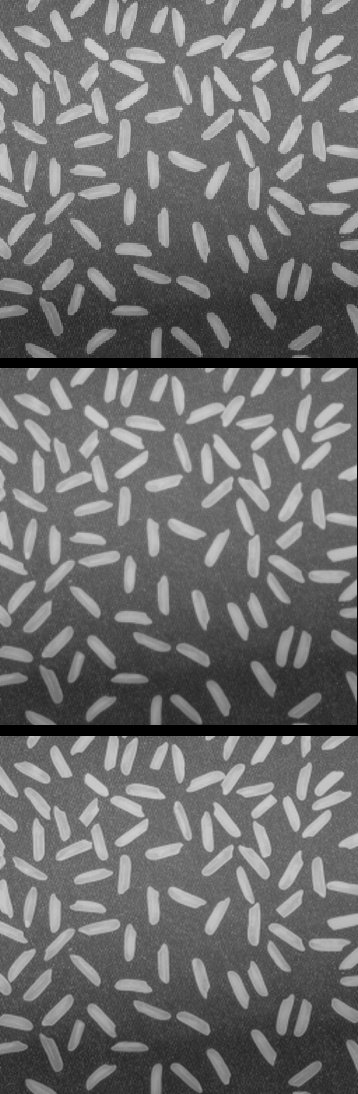
\includegraphics[width=0.3\linewidth]{concatenated_image_big.jpg}
    \caption{big 1.Nearest 2.bilinear 3.bicubic}
    \label{fig:enter-label}
\end{figure}

\begin{figure}[h]
    \centering
    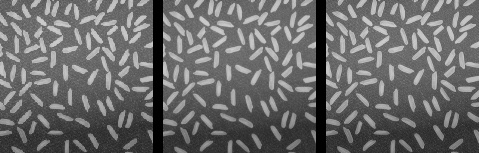
\includegraphics[width=0.5\linewidth]{concatenated_image_small.jpg}
    \caption{small 1.Nearest 2.bilinear 3.bicubic}
    \label{fig:enter-label}
\end{figure}
\begin{figure}[h]
    \centering
    \includegraphics[width=1\linewidth]{time.png}
    \caption{Enter Caption}
    \label{fig:enter-label}
\end{figure}
\FloatBarrier
\section*{Conclusion}
In this experiment, I have learnt that how an image is reshaped and manually run some code to test those interpolation algorithm. Interpolation is a effective tool to process an image to what we want it to be like. However, this process often loss some information so that after many times resize, it may become unreadable. Therefore, interpolation for resizing should only do a limited time. In a word, Interpolation design should consider time cost and spacial cost. Some algorithm may run fast but losing more information. Different environment can apply different algorithm to meet their requirement.   

\end{document}

